\clearpage
\section{Computing larger chains and larger subsystems step by step}
\label{sec:extension}
\subsection{Step 1: choose both physical length scales}
\label{sec:large-scales}
The small-interval expansion concerns an interval short compared with the
whole system, while a continuum description also requires that interval
to contain many lattice spacings. With lattice spacing set to one, these
are the two conditions $\ell/N\ll1$ and $\ell\gg1$. Increasing $N$ at
fixed $\ell=1$ only addresses the first condition. We retain the
six-to-ten-site intervals for all current fits and figures. The previous reference grid was
\begin{align}
 \mathcal N={}&\{32,48,64,82,96,112,128\}\notag\\
 &{}\cup\{144,160,176,192,208,224,240,256\},\notag\\
 &N\in\mathcal N,\qquad \ell\in\{6,7,8,9,10\},\qquad x=\ell/N.
 \label{eq:large-grid}
\end{align}
The symbol $\mathcal N$ denotes this reference subset;
$N=82$ is used literally. Each CFT has $15\times5=75$ retained geometries on this subset; the 30 additional $\ell=4,5$ geometries remain archived. The new active grid is Eq.~\eqref{eq:extended-grid}.
The historical comparison on that subset used the windows
\begin{equation}
 x\leq x_{\rm fit}=0.08\quad\hbox{for fitting},\qquad
 x\leq x_{\rm show}=0.20\quad\hbox{for figures}.
 \label{eq:fit-display-windows}
\end{equation}
On this reference subset there are 51 fitted and 70 displayed observations per directed pair.
The smallest retained ratio is $6/256=0.0234375$; the largest fitted and
displayed ratios are $5/64=0.078125$ and $9/48=0.1875$,
respectively. The sampled grid contains no point between $5/64$ and
the historical fitting cutoff. The active mixture fits instead use
the CFT-wide windows in Eq.~\eqref{eq:common-fit-windows} on the
extended grid. The small-Ising cutoff excludes the reference subset,
whereas the wider small-boson window includes part of it. Increasing $N$ at fixed $\ell=6,\ldots,10$
improves the small-$x$ range while retaining the same lattice resolution;
it does not by itself remove finite-$\ell$ cutoff effects.

\subsection{Step 2: identify the matrix that must be computed}
\label{sec:large-target-matrix}
For a normalized primary state $\ket{\psi_a^{(N)}}$, split the spin basis
into an interval configuration $u$ on $A=\{0,\ldots,\ell-1\}$ and an
environment configuration $y$ on its complement $B$. If
$\Psi_a(u,y)=\langle u,y|\psi_a^{(N)}\rangle$, the exact partial trace is
\begin{equation}
 (\rho_{a,A})_{uv}=\sum_y\Psi_a(u,y)\Psi_a(v,y)^*,\qquad
 \Tr\rho_{a,A}=1.
 \label{eq:large-partial-trace}
\end{equation}
We need the full interval matrix, including its off-diagonal entries,
because the equal mixture and directed relative entropy are
\begin{equation}
 \mu_{ab,A}=\tfrac12(\rho_{a,A}+\rho_{b,A}),\qquad
 D_{a\mid b}=\Tr\rho_{a,A}\log\rho_{a,A}
              -\Tr\rho_{a,A}\log\mu_{ab,A}.
 \label{eq:large-target}
\end{equation}
The logarithm is natural and $p=1/2$. A full-chain vector has $2^N$
entries, whereas $\rho_{a,A}$ has dimension only $2^\ell$, at most 1024
here. The next two steps evaluate Eq.~\eqref{eq:large-partial-trace}
without constructing that vector: fermion covariance matrices for Ising,
and an exact sum of Jastrow amplitudes for the compact boson.

\subsection{Step 3: obtain the Ising interval matrix from its primary sector}
\label{sec:large-ising}
The ingredients are the Jordan--Wigner solution in
Ref.~\cite{Montes2017}, Sec.~VIII and Appendix C, and Gaussian
reduction in Ref.~\cite{PeschelEisler}, Sec.~3.3(II).
The states remain those specified in Sec.~\ref{sec:ising-production},
with independent validation in Appendix~\ref{sec:state-comparisons}.
To make the large-chain calculation explicit,
start from $H=-\sum_jX_jX_{j+1}-\sum_jZ_j$ with periodic spin boundaries.
The Jordan--Wigner Majoranas are
$a_{2j}=(\prod_{k<j}Z_k)X_j$ and
$a_{2j+1}=(\prod_{k<j}Z_k)Y_j$. They obey
$\{a_r,a_s\}=2\delta_{rs}$ and give
\begin{equation}
 H=\frac i4\sum_{r,s=0}^{2N-1}\mathcal A_{rs}a_ra_s,
 \quad \mathcal A_{r,r+1}=2,\quad
 \mathcal A_{2N-1,0}=-2P,\quad \mathcal A^T=-\mathcal A,
\end{equation}
where $P=\prod_jZ_j=\pm1$ is the global parity. All other independent
entries vanish. The following operations determine the state and its reduction.
\begin{enumerate}
\item \textbf{Select the primary and diagonalize the quadratic Hamiltonian.}
For $I,\eps$ take $P=+1$, which gives antiperiodic fermions; for
$\sigma$ take $P=-1$, which gives periodic fermions. Diagonalize the
Hermitian matrix $i\mathcal A=U\operatorname{diag}(\lambda_\mu)U^\dagger$.
For $I$, use signs $\nu_\mu=\operatorname{sgn}\lambda_\mu$.
For $\eps$, reverse the signs of the two smallest positive modes and
their negative-energy partners. This occupies the quasiparticles at
momenta $\pm\pi/N$, with excitation energy $8\sin[\pi/(2N)]$.
\item \textbf{Construct the real covariance and fix the spin state.}
Set $G=\operatorname{Re}[iU\operatorname{diag}(\nu_\mu)U^\dagger]$;
its off-diagonal entries are $G_{rs}=\langle ia_ra_s\rangle$.
In the periodic sector, initially set $\nu_\mu=0$ on the zero modes,
choose real orthonormal null vectors $u,v$ of $\mathcal A$, and add
$\pm(uv^T-vu^T)$. Choose the sign giving $(-1)^N\operatorname{Pf}(G)=-1$.
This resolves the zero-mode occupation and produces the required pure
odd-parity $\sigma$ state. Check $G^T=-G$ and $G^2=-\id$.
The independent finite-chain energy checks are
\begin{equation}
 E_I=-2\csc\frac\pi{2N},\quad E_\sigma=-2\cot\frac\pi{2N},\quad
 E_\eps=E_I+8\sin\frac\pi{2N},\quad
 E=\tfrac14\sum_{rs}\mathcal A_{rs}G_{rs}.
\end{equation}
\item \textbf{Restrict to the interval and reconstruct its density matrix.}
Take $G_A=G_{0:2\ell,0:2\ell}$. A real Schur decomposition gives an
orthogonal matrix $O$ such that
\begin{equation}
 O^TG_AO=\bigoplus_{j=0}^{\ell-1}
 \begin{pmatrix}0&g_j\\-g_j&0\end{pmatrix},\qquad |g_j|\leq1.
\end{equation}
Define interval Majorana matrices using the same spin strings, and
rotate them as $b_r=\sum_sO_{sr}a_s$. The commuting operators
$ib_{2j}b_{2j+1}$ have eigenvalues $\pm1$; therefore
\begin{equation}
 \rho_{a,A}=2^{-\ell}\prod_{j=0}^{\ell-1}
      [\id+g_j i b_{2j}b_{2j+1}].
 \label{eq:large-ising-rdm}
\end{equation}
Each factor supplies probabilities $(1\pm g_j)/2$ for one canonical
mode, so the product is normalized and has the required covariance.
It is the unique Gaussian reduction of the chosen primary.
Because the interval starts at site zero, all its Jordan--Wigner strings
lie inside $A$, making this also the spin reduced density matrix.
\end{enumerate}
The largest full covariance has dimension 512. The global spectral step
has cubic cost and quadratic storage in $N$, while reconstructing
Eq.~\eqref{eq:large-ising-rdm} depends exponentially on $\ell$, not $N$.
We compute the ten-site reduction once for each state and obtain every
smaller requested interval by the further partial trace in
Sec.~\ref{sec:interval-entropy}.

\subsection{Step 4: sum the compact-boson amplitudes exactly}
\label{sec:boson-contraction}
Direct enumeration of $\binom NM$ occupation configurations becomes
impractical as $N$ increases. We instead sum the same Jastrow amplitudes
algebraically. This changes the contraction algorithm, not the primary
state or its endpoint convention. Pfaffian expressions for diagonal
observables in the Haldane--Shastry Jastrow state are established in
Ref.~\cite{Stephan}, Appendix A.1, Eqs.~(A5)--(A11), and Appendix A.2,
Eqs.~(A14)--(A15). The off-diagonal reduced-state formula in
Eq.~\eqref{eq:pf-rdm} is an
implementation derivation in this report. 

Here are the steps in a form that specifies every matrix used in the calculation.
The three charge codes are $(a,b)=(0,0),(1,1),(3,1)$; $M=(N-a-b)/2$ is
the number of occupied sites. To specify one basis configuration
$\ket{n_0\cdots n_{N-1}}$, with $n_j=0,1$, it suffices to list the sites
whose bit is one. This list is the \emph{occupied set}
\begin{equation}
 O=\{j\in\{0,\ldots,N-1\}:n_j=1\},\qquad
 |O|=\sum_{j=0}^{N-1}n_j=M.
 \label{eq:occupied-set}
\end{equation}
Thus $O$ contains site indices, and $|O|$ denotes their number. In the
boson spin convention $s_j=2n_j-1$, ``occupied'' means $s_j=+1$. For
example, on an illustrative six-site chain, $\ket{010101}$ has
$O=\{1,3,5\}$ and $M=3$, with sites numbered from zero.
Every allowed configuration corresponds to one subset of $M$ sites;
this is why there are $\binom NM$ amplitudes.

The coordinate of site $j$ is $z_j=e^{2\pi i j/N}$.
Write the unnormalized coefficient of the basis configuration specified
by $O$ as
\begin{equation}
 P(O)=\Delta(O)^2\prod_{j\in O}z_j^{a+1}g(z_j),\quad
 \Delta(O)=\prod_{i<j\in O}(z_j-z_i),\quad
 g(z)=(1-z/W)^b,\quad W=10^8.
 \label{eq:pf-amplitude}
\end{equation}
This is the polynomial form of the previously validated vertex block.
Let the interval be $A=\{0,\ldots,\ell-1\}$ and its complement be $B$.
With $Z=\sum_{|O|=M}|P(O)|^2$, the normalized amplitude is
$\Psi(O)=P(O)/\sqrt Z$. To label a matrix element, let $U,V\subset A$
be the occupied sets of its row and column configurations, respectively,
and let $Y\subset B$ be the occupied set in the traced-out environment.
The two full-chain configurations are therefore $U\cup Y$ and $V\cup Y$.
The partial trace uses the same $Y$ in both amplitudes and sums over
all such environment configurations. For $|U|=|V|=k$, fixed total
occupation requires $|Y|=M-k$. Thus Eq.~\eqref{eq:large-partial-trace} becomes
\begin{equation}
 (\rho_A)_{UV}=\frac1Z
 \sum_{\substack{Y\subset B\\|Y|=M-k}}
 P(U\cup Y)P(V\cup Y)^*,\qquad |U|=|V|=k.
 \label{eq:boson-environment-sum}
\end{equation}
For unequal $|U|,|V|$ the matrix element is zero, because no common
environment can satisfy the fixed total occupation $M$. The remaining
steps evaluate this numerator and its normalization without enumeration.

\begin{enumerate}
\item \textbf{Convert the environment sum into a moment matrix.}
Set $w(z)=z^{-2(M-1)}|g(z)|^2$. For indices $r,s=0,\ldots,2M-1$, define
\begin{equation}
 \mathsf A_{rs}=(s-r)\sum_{j=0}^{N-1}w(z_j)z_j^{r+s-1}.
 \label{eq:pf-moment}
\end{equation}
The matrix is antisymmetric. Its Pfaffian, denoted $\operatorname{Pf}$,
is the signed sum over all pairings of its indices; for a $2\times2$
matrix it is the upper-right entry, and its square is the determinant.
The empty Pfaffian is one. A confluent Vandermonde determinant uses
two columns $v(z),v'(z)$ for each summed site, where $v_r(z)=z^r$ and
$v'_r(z)=rz^{r-1}$ (zero at $r=0$). Expanding this determinant and summing
over site subsets gives
\begin{equation}
 Z=\sum_{|O|=M}|P(O)|^2=\operatorname{Pf}(\mathsf A).
 \label{eq:pf-norm}
\end{equation}
Indeed, on the unit circle $|P(O)|^2=\Delta(O)^4\prod_{j\in O}w(z_j)$.
Each summed site supplies a pair of columns, so its contribution to
the moment matrix is $w(z)[v(z)v'(z)^T-v'(z)v(z)^T]$.
This is the discrete weighted form of the confluent-determinant sum in
Ref.~\cite{Stephan}, Appendix A.1. That reference uses $L$ for our site
number $N$, and $N$ for our particle number $M$.

\item \textbf{Remove the interval sites with a small matrix update.}
Let $T$ have columns $v(z_j),v'(z_j)$ for $j\in A$, in site order,
and let $C$ be block diagonal with blocks
$-w(z_j)\begin{psmallmatrix}0&1\\-1&0\end{psmallmatrix}$.
Then $\mathsf A_B=\mathsf A+TCT^T$ sums only the environment sites.
All following small matrices have dimension $2\ell$:
\begin{align}
 K_0&=T^T\mathsf A^{-1}T,& Q&=C^{-1}+K_0,\notag\\
 p_\varnothing&=\operatorname{Pf}(Q)\prod_{j\in A}w(z_j),&
 K_B&=K_0-K_0Q^{-1}K_0.
 \label{eq:pf-small}
\end{align}
Here $p_\varnothing=\operatorname{Pf}(\mathsf A_B)/Z$ is the probability
that the interval is empty; it is a reference for the algebra, not a
conditioning applied to the final physical state. All transposes in
these antisymmetric identities are ordinary transposes.
Equation~\eqref{eq:pf-small} follows from two explicit matrix identities:
\begin{align}
 \mathsf A_B^{-1}
 &=\mathsf A^{-1}-\mathsf A^{-1}TQ^{-1}T^T\mathsf A^{-1},\notag\\
 \frac{\operatorname{Pf}(\mathsf A+TCT^T)}{\operatorname{Pf}(\mathsf A)}
 &=(-1)^\ell\operatorname{Pf}(C)\operatorname{Pf}(Q)
 =\left[\prod_{j\in A}w(z_j)\right]\operatorname{Pf}(Q).
\end{align}
The first identity can be verified by multiplying by $\mathsf A_B$;
left and right multiplication by $T^T,T$ gives the stated $K_B$.
In the second, $\operatorname{Pf}(C)=(-1)^\ell\prod_jw(z_j)$.
The empty-interval probability is nonzero on the grid, so the reference
inverse exists even when some individual occupation blocks are small.

\item \textbf{Retain the bra and ket configurations explicitly.}
An interval matrix element is labelled by occupied sets $U,V\subset A$.
It vanishes unless $|U|=|V|=k$, because the global particle number is fixed.
Set $m_j=\mathbf1_{j\in U}+\mathbf1_{j\in V}$. A site with $m_j=1$
selects its evaluation column in $T$; one with $m_j=2$ selects both its
evaluation and derivative columns. Denote the resulting ordered column
indices by $I_{UV}$ and define
\begin{equation}
 \Delta_{UV}=\prod_{i<j\in A}(z_j-z_i)^{m_i m_j}.
\end{equation}
The exact normalized reduced-state element is
\begin{equation}
 (\rho_A)_{UV}=
 P(U)P(V)^*\!\prod_{v\in V}z_v^{-2(M-k)}
 \frac{(-1)^k p_\varnothing
 \operatorname{Pf}[(K_B)_{I_{UV},I_{UV}}]}{\Delta_{UV}}.
 \label{eq:pf-rdm}
\end{equation}
To see the phase and powers, write the common occupied environment as
$Y\subset B$, $|Y|=M-k$. The product of amplitudes factors as
\begin{align}
 P(U\cup Y)P(V\cup Y)^*
 &=P(U)P(V)^*\prod_{v\in V}z_v^{-2(M-k)}
 \Delta(Y)^4\prod_{y\in Y}w(z_y)\notag\\[-2pt]
 &\quad\times\prod_{u\in U,\,y\in Y}(z_u-z_y)^2
 \prod_{v\in V,\,y\in Y}(z_v-z_y)^2.
 \label{eq:pf-factorization}
\end{align}
The fixed columns for $U,V$ and the paired columns for $Y$ give a
confluent Vandermonde determinant with an extra factor $\Delta_{UV}$.
For clarity, let $T_{UV}$ consist of those fixed columns and let
$\mathcal S_{UV}$ denote the sum of the environment-dependent factors
on the right-hand side of Eq.~\eqref{eq:pf-factorization}. Summing each remaining
column pair gives the bordered Pfaffian identity
\begin{align}
 \Delta_{UV}\mathcal S_{UV}
 &=(-1)^k\operatorname{Pf}
 \begin{pmatrix}\mathsf A_B&T_{UV}\\-T_{UV}^T&0\end{pmatrix}\notag\\
 &=(-1)^k\operatorname{Pf}(\mathsf A_B)
       \operatorname{Pf}(T_{UV}^T\mathsf A_B^{-1}T_{UV}).
 \label{eq:pf-bordered}
\end{align}
The first equality is the same pairing expansion as
Eq.~\eqref{eq:pf-norm}, with $2k$ unsummed columns; moving these fixed
columns to the end produces $(-1)^k$. The second follows by block
elimination with determinant-one triangular matrices. Substituting
$K_B=T^T\mathsf A_B^{-1}T$ and
$\operatorname{Pf}(\mathsf A_B)/Z=p_\varnothing$ yields
Eq.~\eqref{eq:pf-rdm}. Thus both off-diagonal phases and normalization
are carried through the environment sum explicitly.
The Pfaffian elimination uses
$\operatorname{Pf}(BAB^T)=\det(B)\operatorname{Pf}(A)$, given in
Ref.~\cite{Wimmer}, Eq.~(5); this identity also fixes the sign rather
than extracting a square root of a determinant.

\item \textbf{Exploit the roots of unity and check precision.}
The identity $\sum_jz_j^n=N$ when $n$ is a multiple of $N$, and zero
otherwise, makes $\mathsf A R$ tridiagonal; $R_{rs}=\delta_{r,2M-1-s}$
reverses the basis order. Put $L=2M-1$. Its nonzero entries are
\begin{align}
 (\mathsf A R)_{rr}&=N(L-2r)(1+b/W^2),\notag\\
 (\mathsf A R)_{r,r+1}&=(\mathsf A R)_{r+1,r}
 =-N(L-2r-1)b/W.
\end{align}
Solving this tridiagonal system gives $\mathsf A^{-1}T$ without a dense
inverse. Only the $2\ell$ matrices and Pfaffians in
Eq.~\eqref{eq:pf-small} remain. For fixed $\ell\leq10$, the dependence
on $N$ is linear; the dependence on interval length is still exponential.
At $\ell=10$ the same principal Pfaffian appears in many bra--ket
pairs. We compute it once and reuse it. For an ordered even index set
$I=\{i_1,\ldots,i_{2k}\}$, the recursion is
\begin{equation}
 f(I)=\sum_{j=2}^{2k}(-1)^j(K_B)_{i_1i_j}
 f(I\setminus\{i_1,i_j\}),\qquad f(\varnothing)=1.
\end{equation}
It is the first-row Pfaffian expansion in Ref.~\cite{Wimmer}, Eq.~(4),
with memoization added here. The denominator
$\Delta_{UV}$ and the Pfaffian depend on the site multiplicities, so
their ratio is also reused for pairs with identical $U\cup V,U\cap V$.
There are at most $(3^\ell+1)/2$ even multiplicity patterns; intermediate
index sets in the recursion are cached separately. This reduces repeated
work without changing Eq.~\eqref{eq:pf-rdm}.
The reference calculation through $N=256$ uses 100 decimal digits internally to handle cancellation in
the empty-interval update and Pfaffian recursion. Before converting to
complex double precision, the trace defect and imaginary part of every
diagonal element must be below $10^{-25}$. Neither a normalization repair
nor eigenvalue clipping is used to pass this check. Independent 130-digit
calculations test the final output accuracy. No sampling or Gaussian
approximation of the boson state is used.
\end{enumerate}

\subsection{Step 5: reduce shorter intervals and evaluate the mixture}
\label{sec:interval-entropy}
The ten-site matrix from either model contains every requested smaller
interval. With site zero the least significant bit, write a ten-site
configuration as $u+2^\ell h$, where $u$ labels the retained sites and
$h$ the sites to trace out. Then
\begin{equation}
 (\rho_{a,\ell})_{uv}=\sum_{h=0}^{2^{10-\ell}-1}
 (\rho_{a,10})_{u+2^\ell h,\,v+2^\ell h}.
 \label{eq:large-trace-short}
\end{equation}
This makes the matrices at different interval lengths mutually
consistent and avoids repeating the most expensive construction.

To evaluate Eq.~\eqref{eq:large-target} efficiently, use its exact local
symmetry. A global Ising parity eigenstate gives a reduced state
commuting with $P_A=\prod_{j\in A}Z_j$; tracing out $B$ removes terms
of odd local parity. A fixed-number boson state gives a reduced state
commuting with the interval number $Q_A=\sum_{j\in A}n_j$, since the
same environment must occur in its bra and ket. Both primaries and
their mixture therefore have a common direct-sum decomposition
\begin{equation}
 \rho_{a,A}=\bigoplus_q\rho_{a,q},\qquad
 \mu_{ab,A}=\bigoplus_q\mu_q,\qquad
 \mu_q=\tfrac12(\rho_{a,q}+\rho_{b,q}).
\end{equation}
For Ising $q$ labels even/odd parity; for the boson it labels occupation
number $0,\ldots,\ell$. At $\ell=10$, the Ising blocks have dimension
512 and the largest boson block has dimension $\binom{10}{5}=252$.
The blocks are \emph{not} separately normalized: their traces are the
physical probabilities of their symmetry sectors.

Let $r_{a,q,i}$ be the eigenvalues of $\rho_{a,q}$ and diagonalize
$\mu_q=V_q\operatorname{diag}(w_{q,j})V_q^\dagger$. Define
$d_{a,q,j}=(V_q^\dagger\rho_{a,q}V_q)_{jj}$. The complete matrix
relative entropy is
\begin{equation}
 D_{a\mid b}=\sum_{q,i}r_{a,q,i}\log r_{a,q,i}
 -\sum_{q,j}d_{a,q,j}\log w_{q,j}.
 \label{eq:large-block-entropy}
\end{equation}
One diagonalization of each unordered mixture serves both directions:
$d_{b,q,j}=2w_{q,j}-d_{a,q,j}$. This is an exact block evaluation of the
matrix logarithm; the mixture is not assumed Gaussian.

Numerically, use $0\log0=0$ and omit eigenvalues at or below $10^{-15}$.
Reject a primary or mixture eigenvalue below $-2\times10^{-12}$ and
reject a discarded mixture-support weight
$\sum_{q,j:w_{q,j}\leq10^{-15}}d_{a,q,j}$ above $10^{-12}$.
Check Hermiticity, unit total trace, and $0\leq D_{a\mid b}\leq\log2$,
allowing roundoff. The upper bound follows from
$\mu_{ab,A}\geq\rho_{a,A}/2$. Repeating the entropy calculation
with threshold $10^{-16}$ measures sensitivity to the numerical cutoff.

\subsection{Step 6: validate the contraction before interpreting a fit}
\label{sec:large-validation-method}
The validation protocol follows the same chain of operations as the
production calculation: identify the primary, construct its interval
matrix, take shorter partial traces, and evaluate the mixture entropy.
We compare against full-vector reductions where enumeration is feasible,
vary arithmetic precision and eigenvalue thresholds, and compare direct
and symmetry-block evaluations of the same matrix logarithm.
The numerical results, error definitions and tested sizes are collected
in Appendix~\ref{sec:large-sanity}; the independent primary-state
comparisons are in Appendices~\ref{sec:boson-sanity} and
\ref{sec:state-comparisons}. These checks assess finite-lattice numerical
accuracy. The new $N=256$ endpoint is checked before generating the
intervening sizes. Its covariance has $512\times512$ entries, and its
interval matrix still has only $1024\times1024$ entries at $\ell=10$.
For the boson, the moment solve grows with $N$ while the cached minors
depend on $\ell$. The 100-digit production contraction is compared
with 130 digits at the new endpoint. These checks and the additional
production diagnostics are reported in Appendix~\ref{sec:n256-sanity}.
The following step addresses the separate comparison with CFT.

\subsection{Step 7: compare with the small-interval prediction}
\label{sec:large-cft-comparison}
To compare each datum with the leading CFT prediction without adding a
fitting law, define the dimensionless ratio
\begin{equation}
 R_{a\mid b}(N,\ell)=
 \frac{D_{a\mid b}(N,\ell)}{c_\alpha^{\rm CFT}(\ell/N)^\alpha}.
 \label{eq:small-x-ratio}
\end{equation}
The CFT leading term corresponds to $R=1$. Increasing $\ell$ at fixed
$N$ changes both the lattice cutoff sensitivity and $x$, so the ratio
need not move monotonically toward one. The retained curves in
Fig.~\ref{fig:small-x} compare $\ell=6,\ldots,10$ at each size.
Doubling $N$ reduces $x$ at fixed interval length; the remaining
variation with $\ell$ shows why smaller $x$ alone does not establish
the continuum coefficient. The excluded $\ell=4,5$ values remain
in the raw data and do not appear in the figures or tables.

A complementary comparison holds $x$ fixed and scales both lengths.
The following directly computed ratios all have $x=1/16$:
\begin{center}
\begin{tabular}{rrrr}\toprule
$N$ & $\ell$ & Ising $R_{\sigma\mid\eps}$ & Boson $R_{ss\mid3s,s}$\\\midrule
32&2&1.09914&0.78366\\
96&6&1.22690&0.97729\\
128&8&1.23071&0.98529\\
160&10&1.23216&0.98886\\\bottomrule
\end{tabular}
\end{center}
The first row is a historical reference and is excluded from the present
fit. The successive changes shrink for both pairs. For Ising the values
stabilize away from one: convergence with lattice resolution at fixed
$x$ need not equal the leading term alone. A coarse interval can appear
closer to that term because lattice and higher-order corrections partly
cancel. These observations motivate the larger-subsystem selection;
they do not specify a functional form for a lattice correction.

The active analysis uses the extended grid of Eq.~\eqref{eq:extended-grid}
with free powers, $F_1$, and $F_2$. Section~\ref{sec:fits} specifies
estimation, residuals and size cross-validation. No missing analytical
subleading coefficient is derived or declared zero.

\begin{figure}[p]\centering
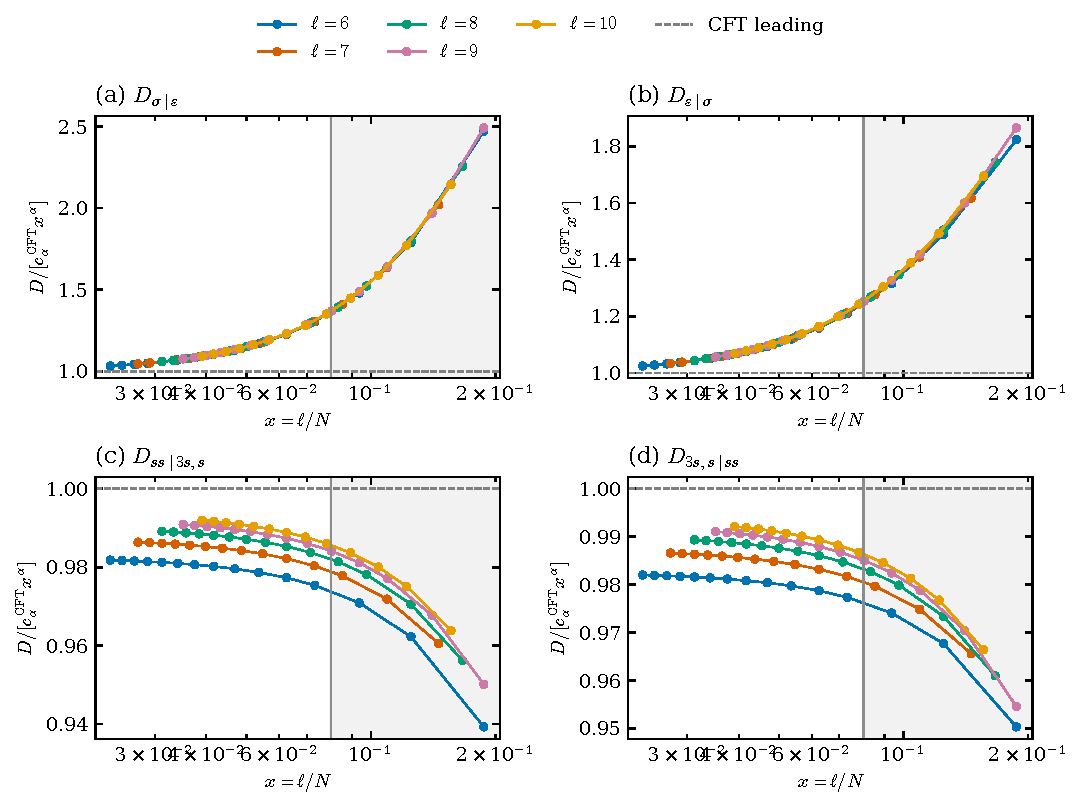
\includegraphics[width=.98\linewidth]{../figs/small_x_diagnostics.pdf}
\caption{Historical smaller-$x$ comparison, without fitting a lattice correction.
The ordinate is $R$ in Eq.~\eqref{eq:small-x-ratio}, with $\alpha=2$,
$c_2^{\rm CFT}=\pi^2/48$ in (a,b), and $c_2^{\rm CFT}=\pi^2/6$ in (c,d).
All data use $p=1/2$, natural logarithms, the 15 sizes through $N=256$
in Eq.~\eqref{eq:large-grid}, $\ell=6,\ldots,10$, and
$\ell/N\leq0.20$. Colors identify fixed $\ell$; line segments only connect
the computed sizes, not fitted curves. The horizontal dashed line is the
CFT leading prediction. Ising uses the critical periodic Hamiltonian
$H=-\sum XX-\sum Z$ and exact covariance matrices; the boson uses
charge codes $(1,1),(3,1)$, $q=2$, $z_j=e^{2\pi i j/N}$, $w_1=0$,
$W=10^8$, and the same normalized vertex/Jastrow states as the original
method. The small-$x$ ends of the curves compare intervals containing
different numbers of lattice sites; every panel contains 70 observations.
The vertical line marks $x_{\rm fit}=0.08$ and the shaded region contains
data excluded from fitting. The ratios themselves use no fitted parameters.}
\label{fig:small-x}
\end{figure}

\subsection{Step 8: extend the chain while retaining numerical precision}
\label{sec:extended-production}
\begin{equation}\mathcal D=\{2\operatorname{round}[30\,100^{j/48}]:j=0,\ldots,48\},\qquad \mathcal R=\{200+4j:j=0,\ldots,200\}.\label{eq:dense-grid}\end{equation}
\begin{align}
\mathcal N_{\rm ising}&=\mathcal N\cup\mathcal D\cup\mathcal R\cup\{4096+256j:j=0,\ldots,16\}\nonumber\\
&\quad\cup\{152,1024,1118,1146,1232,1356,1492,1528,1604,1644\}\nonumber\\
&\quad\cup\{1808,1852,1972,2048,2190,2354,2412,2654,2890,3000\}\nonumber\\
&\quad\cup\{3140,3216,3294,3436,3500,3552,3606,3660,3784,3854\}\nonumber\\
&\quad\cup\{3926,4000,4158,4222,4286,4426,4670,4734,4798,5000\}\nonumber\\
&\quad\cup\{5246,5310,5542,5758,6270,6526,6782,7038,7294,7550\}\nonumber\\
&\quad\cup\{7806,8000,8016,8032,8048,8064,8080,8096,8112,8128\}\nonumber\\
&\quad\cup\{8144\},\nonumber\\
\mathcal N_{\rm boson}&=\mathcal N\cup\mathcal D\cup\{100,104,168,292,322,354,428,472,512,762\}\nonumber\\
&\quad\cup\{924,1024,1118,1356,1492,1644,1808,2048,2412,2922\}\nonumber\\
&\quad\cup\{3540,3750,3916,4096,4234,4376,4608,4720,4834,5000\}\nonumber\\
&\quad\cup\{5222,5626,5810,6250,6466,6688,6918,7156,7402,7656\}\nonumber\\
&\quad\cup\{7920,8192,8436,8688,8948,9216,9462,9714,9974,10240\}\nonumber\\
&\quad\cup\{10488,10740,10998,11264,11764,12288,12800,13312,13814,14336\}\nonumber\\
&\quad\cup\{14840,15360,15864,16384\}.
\label{eq:extended-grid}\end{align}
All indices $j$ in these set definitions are integers within the stated bounds.

The earlier grid in Eq.~\eqref{eq:large-grid} remains a reference subset.
The active mixture fits use Eq.~\eqref{eq:extended-grid}; no intervals
longer than ten sites are added. The primary-to-primary sanity check
in Appendix~\ref{sec:primary-relative-entropy} retains its original
$N\leq256$ grid. The methods below change how the same finite-chain
states and entropies are evaluated, not their definitions.

\subsubsection{Fourier construction and local Ising transition solves}
At criticality the Majorana matrix is uniform apart from its boundary
twist, so its eigenmodes are known Fourier waves. Let $L=2N$ count
Majoranas, with indices $j=0,\ldots,L-1$, and set
$k_m=2\pi(m+t)/L$. The twist is $t=1/2$ for $I,\eps$ and $t=0$
for $\sigma$. Define $w_m=-\operatorname{sgn}(\sin k_m)$.
For the energy state reverse $w_m$ at $m=0,N-1,N,L-1$.
For the spin state set the two zero-mode weights $w_0,w_N$ to zero
and supply their parity explicitly. Then
\begin{equation}
 (\Gamma_a)_{ij}=\frac{i}{L}\sum_{m=0}^{L-1}w_m
 e^{ik_m(i-j)}+\begin{cases}
 [(-1)^i-(-1)^j]/L,&a=\sigma,\\0,&a=I,\eps.
 \end{cases}
 \label{eq:fourier-covariance}
\end{equation}
The imaginary notation in the Fourier sum yields a real antisymmetric
matrix. The last term is $vu^T-uv^T$, with $u_j=L^{-1/2}$ and
$v_j=(-1)^jL^{-1/2}$; it selects the same odd Ramond state as
Sec.~\ref{sec:large-ising}. This is an exact finite-chain construction,
using the free-fermion mode description of Refs.~\cite{Montes2017,PeschelEisler}.
Its energies are
\begin{equation}
 E_I=-2\csc\frac{\pi}{2N},\quad
 E_\sigma=-2\cot\frac{\pi}{2N},\quad
 E_\eps=E_I+8\sin\frac{\pi}{2N}.
 \label{eq:fourier-energies}
\end{equation}
A fast Fourier transform applies $\Gamma_a$ to a vector in
$O(N\log N)$ work. Thus the Hamiltonian eigensolve is unnecessary.

For the anchored transition in Sec.~\ref{sec:complement-ising}, let
$\Gamma'_b$ be the covariance after applying the local anchor.
Form $K=\id-\Gamma_a\Gamma'_b$ by applying the Fourier transform to
batches of columns. Factor the real matrix $K$ once with pivoted LU
(lower and upper triangular factors). Let $E_A$ be the first $2\ell$
columns of the identity. Solve only
\begin{equation}
 KZ=(\id-i\Gamma_a)E_A,\qquad
 \Gamma_{ab,A}=i\{E_A^T(\id-i\Gamma'_b)Z-\id_{2\ell}\}.
 \label{eq:local-transition-solve}
\end{equation}
The real and imaginary right-hand sides reuse the same LU factors.
The anchor overlap is $|\det K|^{1/4}/2^{N/2}$; its logarithm is
obtained from the LU diagonal. Reconstruct the local Gaussian operator
and restore the anchor, exactly as in the earlier Gram calculation.
We never construct a full complex transition covariance or its inverse.
The remaining dense factorization costs $O(N^3)$ arithmetic and the
stored real matrices cost $O(N^2)$ memory. The interval density matrices
still have dimension at most $2^{10}=1024$.

\subsubsection{Direct evaluation of small entropy remainders}
\label{sec:stable-entropy}
At very small fractions, subtracting $\log2-D^B$ or two almost equal
entropy traces loses relative precision. Instead, evaluate their
remainder directly with matrix-function divided differences
\cite{Higham}. The following identity is an algebraic numerical device,
not a CFT expansion or a new analytical entropy coefficient.

Set $f(t)=t\log t$, with $f(0)=0$. In a basis where a positive reference
matrix is $D=\operatorname{diag}(d_i)$, write
$H=D+E=V\operatorname{diag}(\lambda_k)V^\dagger$.
The first-order matrix derivative has diagonal $f'(d_i)E_{ii}$.
For the remainder diagonal, use
\begin{equation}
 \mathcal R_i=[f(H)-f(D)]_{ii}-f'(d_i)E_{ii}
 =\sum_k |(V^\dagger E)_{ki}|^2\,
 \frac{\lambda_k\log(\lambda_k/d_i)-\lambda_k+d_i}
      {(\lambda_k-d_i)^2}.
 \label{eq:stable-remainder}
\end{equation}
To verify it, expand $[f(H)]_{ii}=\sum_k|V_{ik}|^2f(\lambda_k)$,
use $\sum_k|V_{ik}|^2=1$ and
$E_{ii}=\sum_k|V_{ik}|^2(\lambda_k-d_i)$, and factor the scalar
Taylor remainder. Finally,
$(\lambda_k-d_i)V_{ik}=(EV)_{ik}$ converts its squared factor to
the numerator weight in Eq.~\eqref{eq:stable-remainder}.
At equal arguments the quotient is $1/(2d_i)$.
With $u=(\lambda-d)/d$, compute it as
\begin{equation}
 \frac1d\frac{(1+u)\log(1+u)-u}{u^2}
 =\frac1d\sum_{n=0}^{\infty}\frac{(-u)^n}{(n+1)(n+2)}.
 \label{eq:stable-scalar}
\end{equation}
The code uses ten terms only for $|u|<0.02$, where the omitted
tail is below double-precision accuracy, and the closed expression
otherwise. This series stabilizes a scalar matrix-function evaluation;
it is unrelated to a small-interval power-law fit.

For $D$ the eigenvalue matrix of the mixture on $A$ and $H$ the source
state in that basis, equal unit traces give
$S(\rho\|\mu)=\sum_i\mathcal R_i$. For the complement, first define
the local transition $T_{ab}^A=\Tr_B\ket a\bra b$.
The unweighted Gram matrix has blocks
$H=\left(\begin{smallmatrix}\rho_a^A&T_{ab}^A\\
(T_{ab}^A)^\dagger&\rho_b^A\end{smallmatrix}\right)$.
Its relation $H=2\mathcal G^*$ to the weighted Gram matrix is derived
in Sec.~\ref{sec:complement-gram}. Transform the two diagonal blocks
to their separate Schmidt eigenbases and let $D$ contain their
eigenvalues on its diagonal.
Then $E$ contains only the off-diagonal transition blocks, so its
first-order diagonal vanishes. If $P_a,P_b$ select the two state blocks,
the Gram entropy identity gives the deficit
$\delta_{a\mid b}\equiv\log2-D^B_{a\mid b}$ directly:
\begin{equation}
 \delta_{a\mid b}=\Tr P_a[f(H)-f(D)]
       =\sum_{i\in a}\mathcal R_i,\qquad
 \delta_{b\mid a}=\sum_{i\in b}\mathcal R_i.
 \label{eq:stable-deficit}
\end{equation}
Complex conjugating the entire Gram matrix preserves these real block
traces. Thus even a deficit much smaller than machine precision
relative to $\log2$ can be stored accurately on its own.

The identities are exact on a positive support. In double precision
we retain reference eigenvalues above $\tau=10^{-15}$ in each
symmetry sector. The discarded tails are a numerical approximation;
they are checked by varying $\tau$ to $10^{-14}$ and $10^{-16}$ at
every new size for $\ell=4,10$. We additionally compare with the original
trace-log and Gram formulas and with a high-precision, noncommuting
two-dimensional example. These checks, together with the larger-size
state-contraction tests, are reported in Appendix~\ref{sec:scaling-checks}.

\subsubsection{Boson scaling and the practical boundary}
The boson continues to use the exact sparse moment and small Pfaffian
reductions in Sec.~\ref{sec:boson-contraction} and
Appendix~\ref{sec:complement-pf-details}. The dense high-precision
minors depend on $\ell$, not on $N$. At the added sizes the moment
algebra uses 120 decimal digits before its final conversion to double
precision. Independent sampled entries use 160 digits and direct
pivoted Pfaffians instead of cached recursive minors.
Although the physical moment matrices are sparse, the current Python
pivot searches scan remaining indices. Their bookkeeping can cost
$O(N^2)$ time, in addition to the arithmetic and the $O(N\ell)$ stored
right-hand sides. This becomes the main practical obstacle before the
$2^\ell$ interval dimension changes. The measured limits and timings
below refer to this implementation on this machine; they are not
mathematical maximum chain lengths.
\begin{longtable}{lrrrr}
\caption{Measured largest completed chains, with three diagonal states, three transitions, both directions, and every $\ell=4,\ldots,10$. Wall time includes both interval calculations and endpoint cutoff checks. Memory is the process high-water resident set (GiB), not the size of one matrix; it may include allocations retained from preceding stages. The host has 32 GiB RAM. These are validated endpoints, not absolute mathematical limits.}
\label{tab:scaling-resources}\\\toprule
CFT & Largest $N$ & Seconds & Peak GiB & Minimum retained fraction\\\midrule
\endfirsthead
\toprule
CFT & Largest $N$ & Seconds & Peak GiB & Minimum retained fraction\\\midrule
\endhead
\bottomrule\endfoot
ising & 8192 & 93.46 & 9.0882 & $7.324\!\times\!10^{-4}$\\
boson & 16384 & 506.34 & 0.73204 & $3.662\!\times\!10^{-4}$\\
\end{longtable}
For Ising, doubling the largest tested $N$ would multiply the dominant stored matrix sizes by four, giving an estimated 36.4 GiB with the present allocation pattern, above this host\textquotesingle s RAM. The dense LU arithmetic would grow by about eight. For the boson, sparse index scans still permit further growth but become costly: doubling $N$ can quadruple that bookkeeping. Such extrapolations are estimates, not executed benchmarks. No larger size is claimed as validated.


